\section{Media Reader Eiffage}

\begin{figure}[h]
    \centering
    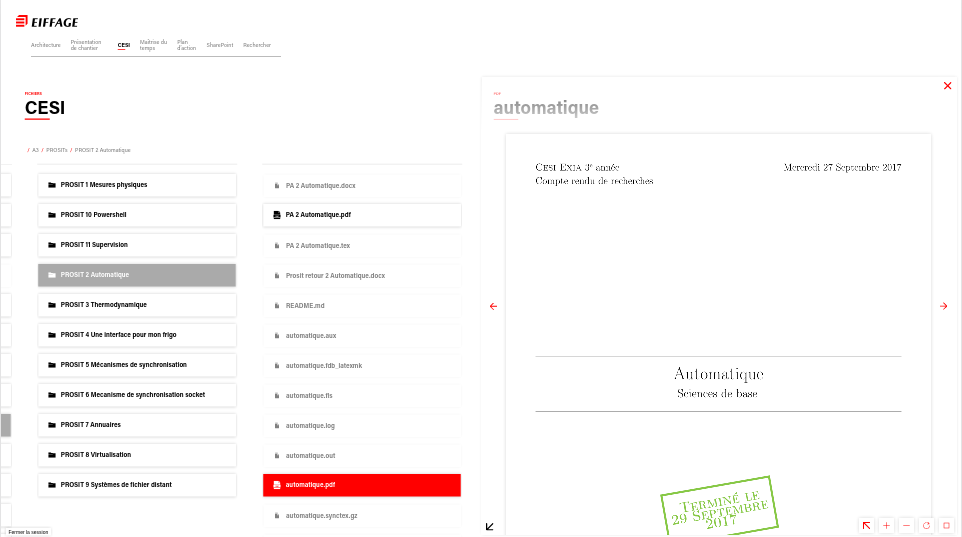
\includegraphics[scale=0.5]{img/media-reader.png}
    \caption{L'interface principale de l'application de lecture des médias Eiffage}
\end{figure}

\subsection{Eiffage}

Eiffage est un grand groupe de traveaux public.
3\up{e} de France, il travaille sur de grands projets dans toute la France.

Dans le cadre de leur chantier de rénovation Laborde, l'objectif était de concevoir une salle de contrôle du chantier connectée.

La salle de contrôle du chantier (appelée salle cockpit) et une salle de réunion des personnes impliquées dans le déroulement du projet de rénovation.
Les plans, les problèmes et les solutions y sont discutés durant toute la durée du projet.
Les plans étudiés sont stockés sur un serveur central et sont disponibles aux employés pour les étudier, les annoter et les commenter.

\medskip

Nous avons mis en place 3 solutions pour ce chantier.

La première est une table tactile sur laquelle il est possible d'ouvrir, de manipuler et d'annoter les plans depuis le serveur central.
Cela vient remplacer les impressions successives de plans pour les annotations et les modifications.
Cela permet de réduire la consommation d'encre et de papier mais aussi de gagner du temps.

La seconde est un écran d'affichage permettant de positionner des Post-its sur un plan.
Ces Post-its sont associés à une personne et définissent les tâches à accomplir.

La dernière solution est un explorateur de fichiers permettant d'afficher des photos, vidéos ou documents du chantier.
Cette solution a pour objectif de permettre une meilleure présentation du chantier avec des documents directement importés depuis le serveur central.

\medskip

Dans ce projet, j'ai notamment travaillé sur le navigateur de fichiers.
Ce navigateur de fichiers est affiché sur un écran de 84 pouces tactile mettant à disposition des employés un formidable outil de présentation.

\begin{figure}[h]
    \centering
    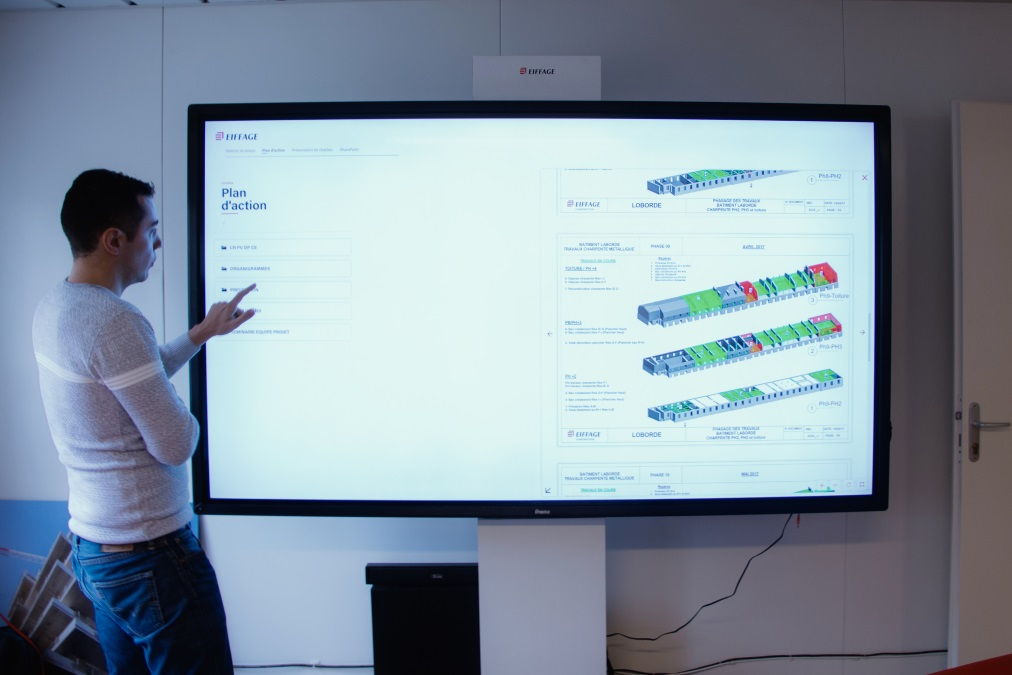
\includegraphics[scale=1.2]{img/media-reader-pres-1.jpg}

    \bigskip

    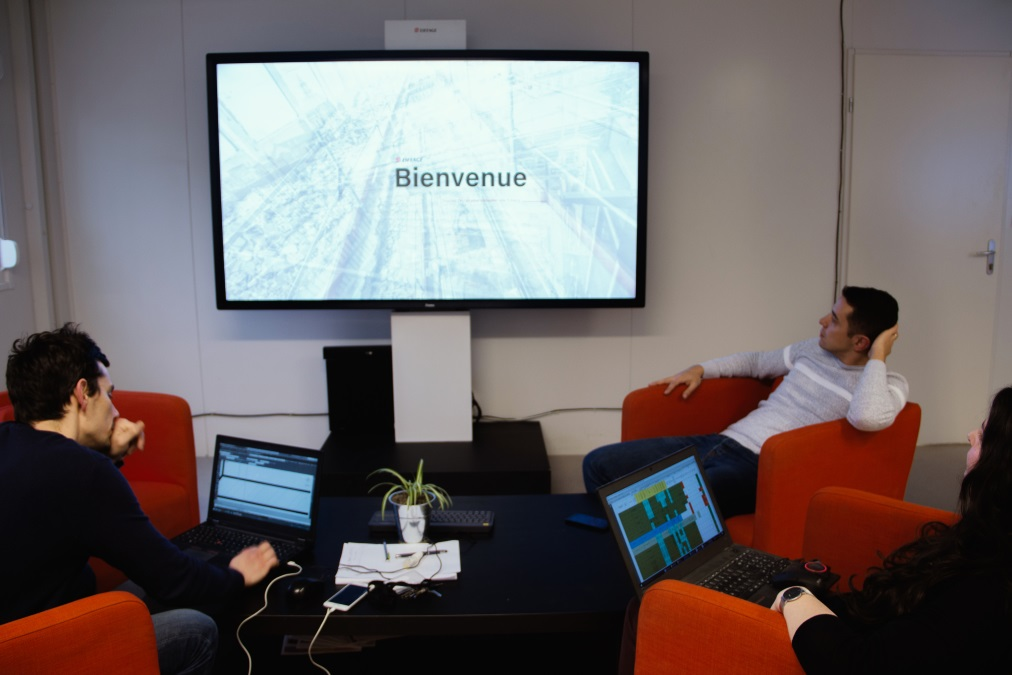
\includegraphics[scale=1.2]{img/media-reader-pres-2.jpg}
    \caption{Un aperçu de l'explorateur de fichiers une fois installé dans la salle cockpit}
\end{figure}

\clearpage

\subsection{Lecteur de médias}

Le lecteur de Media Eiffage doit donc disposer des fonctionnalités suivantes :

\begin{itemize}
    \item Se connecter à un emplacement réseau
    \item Lister le contenu des dossiers et pouvoir naviguer dans l'arborescence
    \item Afficher un aperçu des fichiers images, vidéo et PDF
    \item Intégrer l'application dans un contexte Active Directory où chaque utilisateur doit pouvoir ouvrir sa session personnelle
\end{itemize}

La courte liste des fonctionnalités m'a permis de travailler plus en profondeur sur la structure de l'application et ainsi de développer des fonctionnalités solides.

\subsection{Application existante}

Dû à des retards sur la livraison du matériel requis pour développer les applications Eiffage, le développement était peu avancé.
L'explorateur de fichiers chargeait toute l'arborescence de la source des données ce qui était peu optimisé.
En revanche la solution initiale contenant un navigateur de PDF que j'ai repris dans ma version de l'application.

Globalement, j'ai repris une grande partie de l'application qui n'utilisait pas les WebComponents pour l'adapter aux nouvelles techniques Web permettant de modulariser chaque élément de l'interface.

\subsection{Technologies utilisées}

Pour cette application, j'ai décidé d'utiliser la même technologie que les autres applications de LTBL soit Electron et l'utilisation des WebComponents.

Je n'ai pas utilisé de technologie supplémentaire ni de librairie complémentaire pour me former sur les futures normes Web.

\subsection{Structure}

Avec ce projet, j'ai continué à expérimenter avec les WebComponents pour trouver le bon paradigme d'utilisation.
En effet, les WebComponents présentent une structure d'application très différente des applications Web standard.
Chaque composant étant isolé des autres il faut utiliser des systèmes de communication comme les événements JavaScript pour permettre une communication entre les components.

Pour ce projet, j'ai fragmenté mon code sur de multiples niveaux de WebComponents.
Contrairement à l'application de BioMérieux où j'ai fait de grands composants par grande partie de l'application.
Dans cette application, j'ai modularisé au maximum les éléments de l'interface pour pouvoir réutiliser ces composants dans un autre contexte.

\begin{figure}[h]
    \centering
    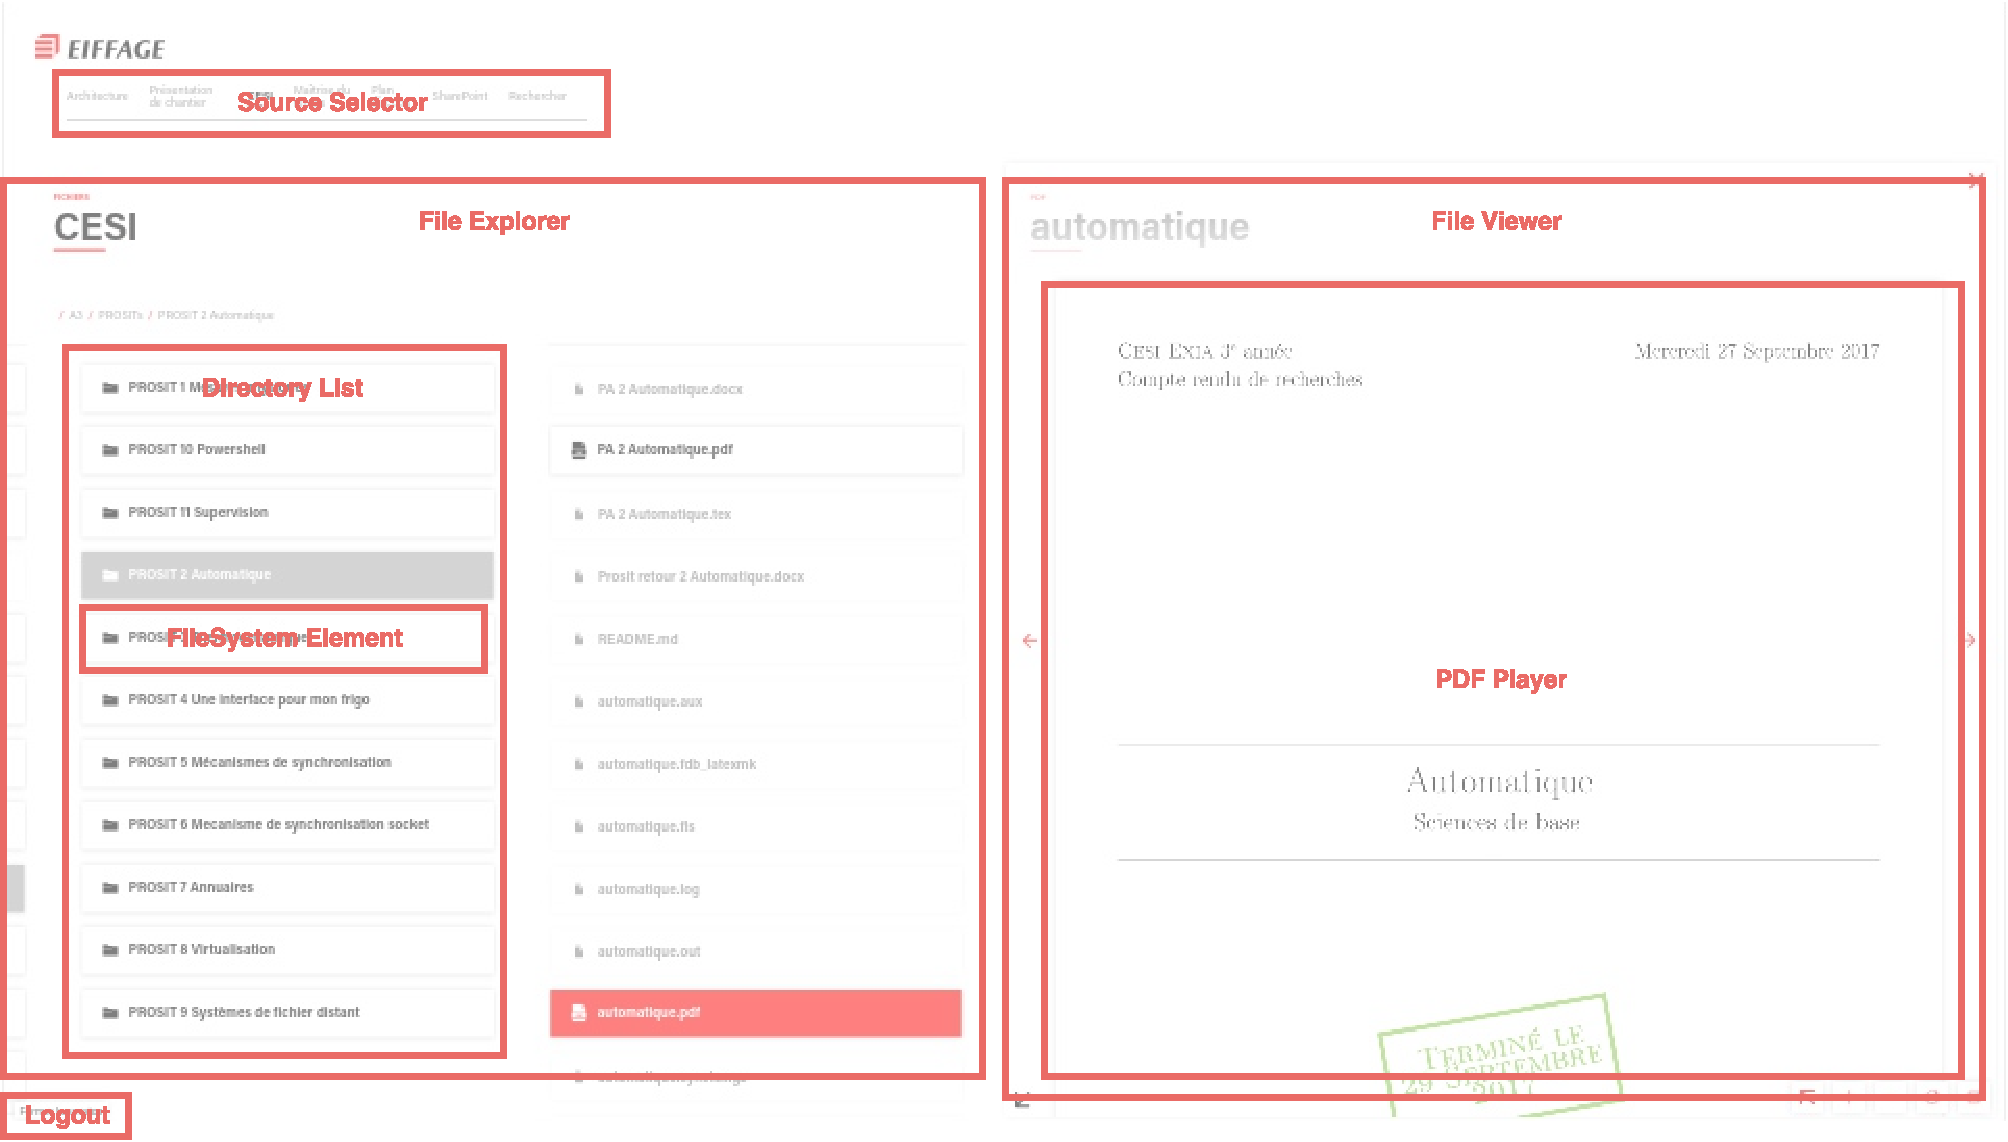
\includegraphics[scale=0.5]{img/media-reader-structure.pdf}
    \caption{La structure de l'application avec les différents components qui composent l'interface}
\end{figure}

Chaque component est séparé des autres et peut fonctionner seul sans nécessiter d'intervention des components parents.

\begin{description}
    \item[Source Selector] Un simple menu de sélection des sources permettant à l'utilisateur de choisir parmi plusieurs éléments disponibles chargés depuis un fichier de configuration général
    \item[File Explorer] Le component principal de l'application, car il permet de naviguer dans les dossiers d'une source et d'ouvrir des fichiers  de cette source
    \item[Folder List] Compris dans le component \textbf{File Explorer}, il va lire le contenu d'un dossier passé en attribut et en lister le contenu
    \item[File System Element] Compris dans le component \textbf{Folder List}, ce component va chercher le fichier ou le dossier passer
    \item en attribut et afficher son titre et son icône
    \item[File Viewer] Ce component assez simple est en charge d'afficher un aperçu d'un fichier passé en attribut et de choisir le bon lecteur pour le type de fichier demandé
    \item[PDF Player] Le lecteur de fichiers, dans ce cas PDF, permettant d'afficher correctement le fichier en fonction de son type; j’ai aussi conçu \texttt{image-player} pour les images et \texttt{video-player} pour les vidéos
    \item[Logout] Un composant conçu par un collègue permettant de se déconnecter de la session Windows actuelle
    \item[Lock Screen] Un component non affiché sur le schéma permettant d'afficher un écran de bienvenue avec un diaporama de photos provenant d'un emplacement réseau en arrière-plan; cet écran de verrouillage s'affiche après une période d'inactivité
    \item[Web Frame] Un composant permettant d'afficher une page Web avec le moteur de rendu webkit
\end{description}

\begin{figure}[h]
    \centering
    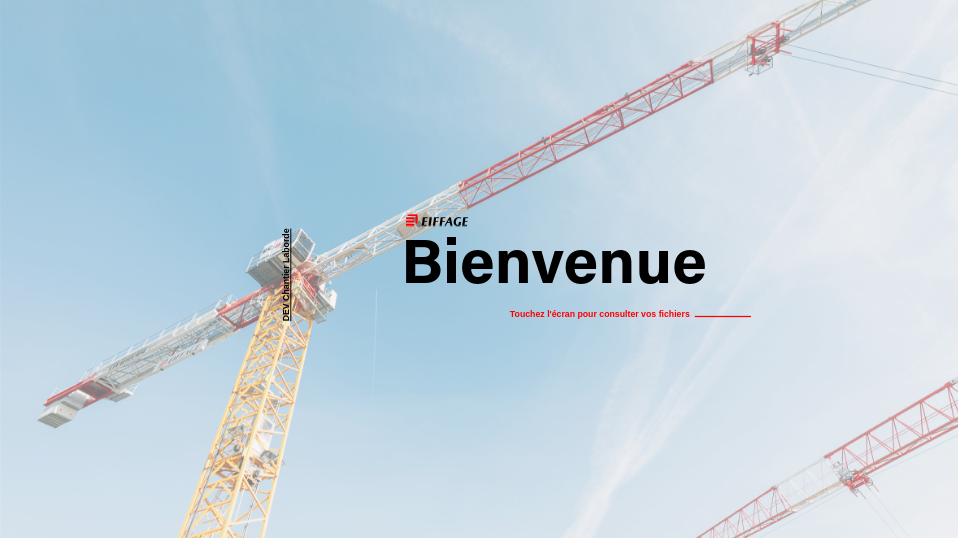
\includegraphics[scale=0.5]{img/media-reader-lock.png}
    \caption{Vue de l'écran de verrouillage du lecteur de médias}
\end{figure}

\subsubsection{Component d'animation}
\label{animationblock}

Les animations prennent une grande place dans le design des applications de LTBL et celles-ci sont prises très au sérieux par l'équipe de développement.
Les animations dans les technologies Web posent quand même un problème.
Elles doivent êtres prises en compte des la création des éléments pour être correctement utilisables.
De plus l'animation des plusieurs éléments les uns a la suite des autres est difficile en CSS.

J'ai donc créé un component Web en charge de gérer les animations.
Un component comme \texttt{Animated Block} permet de ne pas penser à l'animation pendant le développement, mais de l'ajouter à la fin, dès que les fonctionnalités sont ajoutées comme une dernière finition.
Ce component propose un système d'animation se basant sur les transitions CSS (bien plus performantes que les animations JavaScript) et les classes des éléments à animer.

L'\texttt{Animated Block} se présente comme un bloc transparent, qui n'a pas d'incidence sur le style global de l'application.
Il réagit comme un \texttt{div} et peut facilement remplacer un élément de l'interface pour l'animer.

Un \texttt{Animated Block} propose 2 animations par défaut \texttt{enter} et \texttt{leave} servant respectivement a faire apparaître l'élément et a le faire disparaître.
Le component n'impose pas d'animation de base, mais met à disposition système permettant de faire une animation facilement.

Par exemple, prenons l'animation \texttt{enter}.

\begin{figure}[h]
    \centering
    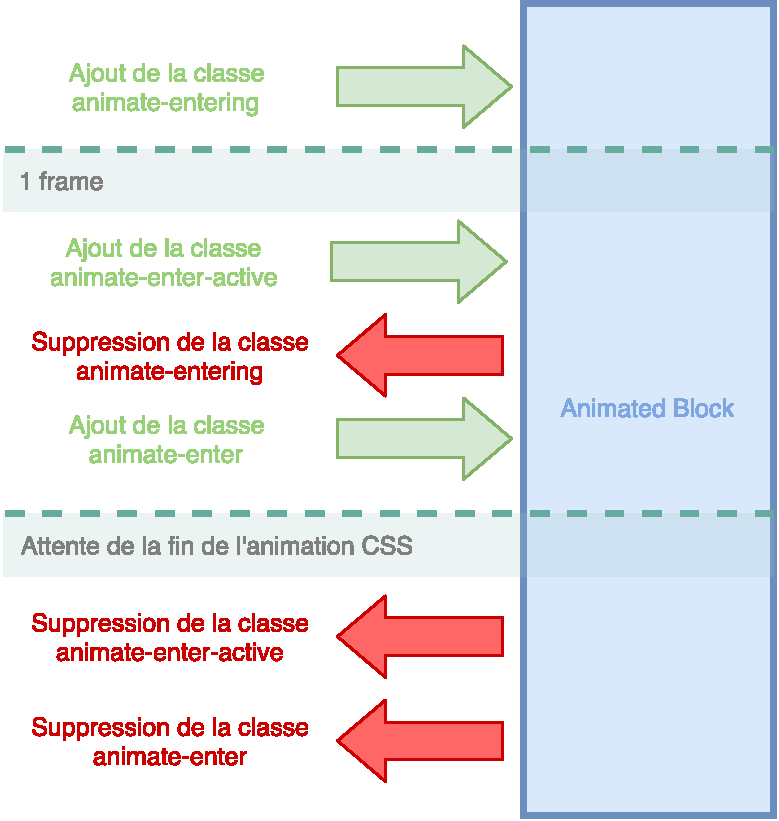
\includegraphics[scale=0.5]{img/animated-block.pdf}
    \caption{Système d'animation d'\texttt{Animated Block}}
\end{figure}

Chaque animation est composée de 3 classes permettant de créer le mouvement correct

\begin{description}
    \item[Classe de setup] En charge de mettre en style l'élément avant l'animation (Ex. placer l'élément hors de l'écran pour le faire apparaître)
    \item[Classe d'animation] Gérant l'animation dans son ensemble, c'est sur cette classe que l'on positionne la propriété de \texttt{transition} CSS permettant d'animer les différents styles de bloc
    \item[Classe d'état final] En charge de définir l'état final de l'élément après l'animation (elle n'est pas nécessaire si l'état final est le même que l'état standard du bloc)
\end{description}

Ainsi, toute l'animation passe par le fait d'ajouter ou de retirer ces classes.
Le pipeline d'animation est alors le suivant :

\begin{enumerate}
    \item On ajoute la classe de setup (\texttt{animate-entering} dans notre cas)
    \item Une frame plus tard (une fois l'élément stylisé), on ajoute la classe d'animation (\texttt{animate-enter-active} dans notre cas)
    \item On retire la classe de setup puis on ajoute la classe d'état final (\texttt{animate-enter} dans notre cas)
    \item On calcul le temps de l'animation puis on attend la fin de celle-ci
    \item On retire la classe d'animation et d'état final
\end{enumerate}

Il est bien sûr possible de créer ses propres animations en spécifiant manuellement les différentes classes à utiliser, mais les deux animations (\texttt{enter} et \texttt{leave}) sont des animations normalisées.

Dès qu'une animation est déclenchée, une promesse est renvoyée pour permettre de savoir quand elle se terminera.
Cela permet d'effectuer des actions après que l'animation soit passée comme réinitialiser des données ou effectuer des actions en arrière-plan.

Enfin, le component \texttt{Animated Block} dispose d'une fonction statique \texttt{animateStack()} permettant d'animer un ensemble d'éléments les uns après les autres en exécutant simplement une fonction.

Ainsi, grâce à ce système, on peut simplement ajouter des animations au projet sans ajouter beaucoup de lignes de code pouvant mener à des bugs.
Il suffit d'appeler la fonction d'animation et d'attendre la résolution de la promesse pour effectuer des actions après l'animation.

\subsubsection{Submodules Git \& Integration}

Sur les 3 projets que nous avions à développer pour Eiffage, les 3 avaient besoin d'un explorateur de fichier.
Que ce soit pour afficher des aperçus comme le projet actuel ou ouvrir un plan sur la table interactive.
L'explorateur de fichiers est un élément essentiel de l'interface.

Et c'est ici que l'on voit l'intérêt d'utiliser des WebComponents.
En effet, il suffit d'utiliser exactement le même code que j'ai utilisé pour le lecteur de médias dans tous les autres projets.

Un autre problème se pose alors.
Il serait contre-productif de faire une copie du code sur chacun des projets et il serait plus intéressant d'utiliser un système de mise à jour automatique.
Cela peut être assuré par les submodules Git.

\begin{figure}[h]
    \centering
    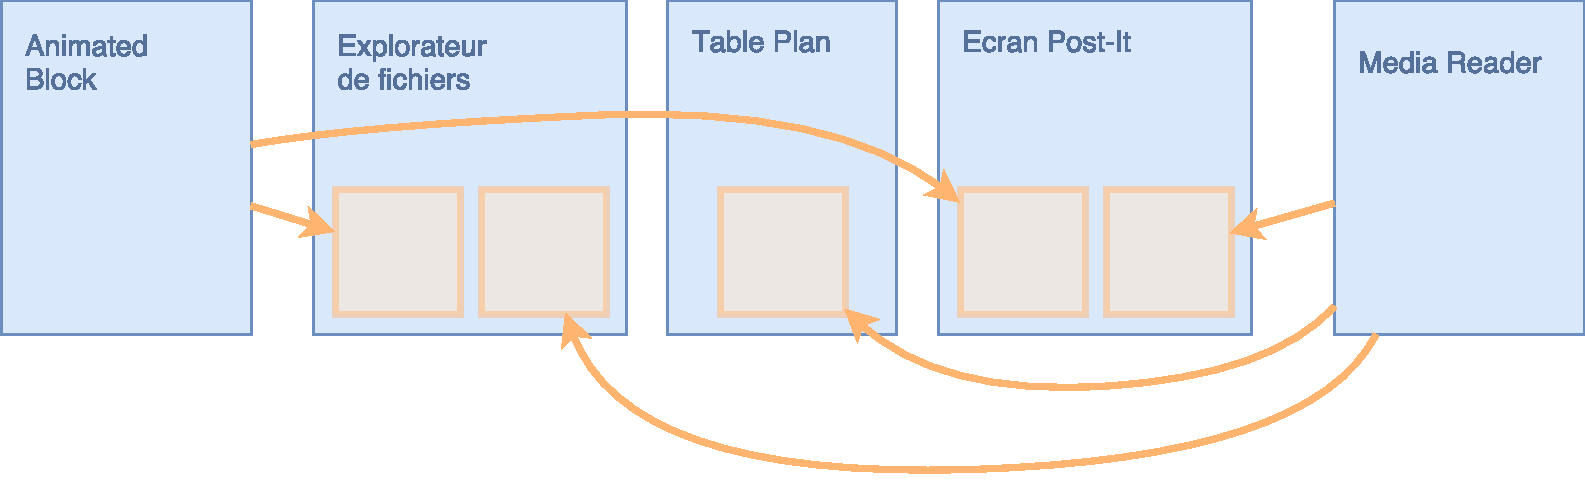
\includegraphics[scale=0.5]{img/submodules.pdf}
    \caption{Exemple d'utilisation des submodules Git}
\end{figure}

Pour tous les projets chez LTBL j'ai utilisé git et BitBucket pour la gestion du code source.
Git dispose d'une fonctionnalité de Submodule.
Cela consiste en un sous-repository dans le projet actuel.
Ce sous-reprository fait référence à un repository en ligne commun à tous les projets.

Ainsi, on peut éditer le code du component partagé sur le repository qui lui est dédié puis, sur les projets en ayant besoin, récupérer les modifications avec \texttt{git pull}.

\subsection{Difficultés \& Ergonomie}

Ce projet m'a amené à travailler sur une interface tactile qui allait être utilisée au quotidien et je devais porter une attention toute particulière à l'ergonomie de l'interface.

J'ai alors eu de nombreuses heures d'expérimentations sur les gestes que peuvent avoir les utilisateurs sur les lecteurs comme celui des PDF .
J'ai ainsi pu me rendre compte de la difficulté d'avoir une réaction ergonomique aux gestes tactiles comme ceux du pincement ou de la rotation à deux doigts.

J'ai donc effectué beaucoup d'expériences avec de nombreux changements de paramètres pour trouver les bonnes valeurs.
Malheureusement, beaucoup de fonctionnalités gestuelles n'ont pas été retenues, car elles n'apportèrent qu'une frustration supplémentaire pour l'utilisateur.

Dans un second temps je me suis aussi heurté au problème des PDF d'Eiffage.
Les plans sont dans ce format et sont générés automatiquement par le logiciel d'architecture.
Il en résulte des documents de très grosse taille et complexe à afficher, ainsi chaque rendu pouvait prendre près de 30 secondes.
Un temps que l'on doit réduire le plus possible pour éviter une attente de la part de l'utilisateur.
Pour réduire ce temps, j'ai mis en place un système qui analyse le zoom effectué et qui ne lance un rendu qu'en cas de zoom important.
Malgré le gain de temps que cela apportait, il fallait trouver une astuce pour éviter les rendus du PDF bien trop lourd.
J'ai alors décidé d'actualiser le zoom du PDF lors du redimensionnement de la fenêtre d'aperçu pour toujours avoir un zoom optimal et réduire le recours au zoom manuel.

\subsection{Installation}

Nous avons installé ce projet sur le site de Laborde près de la garde Saint-Lazare à Paris.
Nous avons installé l'écran de 84 Pouces sur son pied et avons installé l'application sur l'ordinateur de manière globale sur la machine.

Un problème s'est posé quand nous avons pris connaissance des prérequis de sécurité en vogue chez Eiffage.
En effet, Eiffage utilise le système Active Directory et le département Informatique de l'entreprise ne permet pas la création d'un compte spécifique pour l'exécution de l'application.
Il fallait donc faire en sorte que l'application puisse s'exécuter sur n'importe quel utilisateur se connectant.
J'ai alors simplement ajouté un raccourci vers l'application dans le dossier \texttt{Démarrage} du menu démarré global de l'ordinateur pour que l'application se démarre à chaque ouverture de session.
J'ai aussi ajouté un bouton de déconnexion permettant de se déconnecter de la session sans passer par le menu démarrer.

\subsection{Conclusion}

Ce projet m'a permis, au travers d'un sujet simple, de poursuivre ma découverte des WebComponents et des interfaces tactiles.
J'ai rencontré des obstacles qui m'on fait prendre conscience de la difficulté de créer des interfaces tactiles de qualité et le développement de gestes tactiles qui sembles naturels.
Malgré ces problèmes, j'ai réussi à livrer une application fonctionnelle et dont les composants peuvent aisément être intégrés dans les 2 autres projets d'Eiffage qui ont aussi besoin d'un explorateur de fichiers.
